\documentclass[12pt]{article}

\usepackage{sbc-template}
\usepackage{graphicx,url}
\usepackage[utf8]{inputenc}
\usepackage[brazil]{babel}
\usepackage[latin1]{inputenc}  
\usepackage{subfig}
\usepackage{array}

\sloppy

\title{Compilador TPP - Análise léxica}

\author{Caio Eduardo Theodoro}


\address{Universidade Tecnológica Federal do Paraná
  (UTFPR)\\
\nextinstitute
  Campo Mourão, PR -- Brasil\\
\nextinstitute
 Email:
  \email{caio.2001@alunos.utfpr.edu.br}
}

\maketitle
\begin{abstract}
This report describes the lexical analysis for a compiler of the TPP language. The operation of the lexical analyzer will be presented, as well as the description of the tokens and the symbol table.
As part of the work, the results of the scanning and token recognition processes for an example program will be presented.
\end{abstract}
\begin{resumo} 
 Este relatório descreve a análise léxica para um compilador da linguagem TPP. Será apresentado o funcionamento do analisador léxico, bem como a descrição dos tokens e a tabela de símbolos.
 Também como parte do trabalho, será apresentado os resultados do processos de varredura e reconhecimento de tokens para um programa de exemplo.
\end{resumo}

\begin{document} 

\vspace{1cm}
\section{Introdução a análise léxica}

Como primeira etapa do processo de compilação, a análise léxica tem como objetivo identificar os tokens presentes no programa.
Tokens são, basicamente, os elementos que compõem a linguagem, como palavras reservadas, operadores, identificadores, etc. A partir deles é possível reconhecer a estrutura do programa e, consequentemente, realizar a análise sintática e semântica.
Como primeira etapa então anterior á definição dos tokens a serem reconhecidos pelo analisador léxico, temos a definição da linguagem, que será descrita a seguir.

\vspace{1cm}
\section{Definições da linguagem - TPP}

A linguagem TPP é uma linguagem de programação imperativa, isto é, ela é orientada a comandos. Seu suporte a funções, estruturas de controle condicional e de repetição a torna uma linguagem de programação de propósito geral.
O exemplo na Figura \ref{fig:f1} apresenta um programa em C e seu equivalente em TPP. 

 
      \begin{figure}[h!]
        \centering
         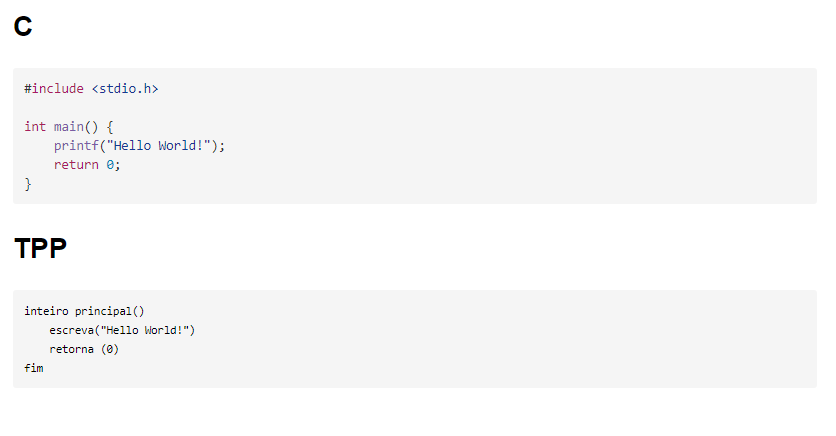
\includegraphics[scale=0.8]{images/c_tpp.png}
        \label{fig:f1}
        \end{figure}

A seguir, serão apresentadas as regras de definição da linguagem.

\vspace{1cm}
\subsection{Palavras reservadas, identificadores e literais}

Serão utilizadas 11 palavras reservadas para realizar a construção do nosso analisador léxico. São elas:


\begin{itemize}
    \item se
    \item então
    \item senão
    \item fim
    \item repita
    \item flutuante
    \item retorna
    \item até
    \item leia
    \item escreva
    \item inteiro
\end{itemize}

Além das palavras reservadas, também serão utilizados identificadores e literais. Identificadores são palavras que podem ser utilizadas para nomear variáveis, funções, etc. Eles devem começar com uma letra e podem conter letras, números e o caractere \textbf{\_} (underscore). Literais são valores constantes que podem ser atribuídos a variáveis. Eles podem ser do tipo \textbf{inteiro, flutuante e notação científica}.


\vspace{1cm}
\subsection{Operadores,delimitadores e comentários}


Serão utilizados 7 operadores ou simbolos para realizar a construção do nosso analisador léxico. Eles e seus respectivos símbolos são:
\vspace{1cm}
\begin{itemize}
    \item Soma: +
    \item Subtração: -
    \item Multiplicação: *
    \item Divisão: /
    \item E lógico (\^): &&
    \item OU lógico (v): ||
    \item Negação lógica (!): !
\end{itemize}

Também serão usados 5 comparadores ou operadores relacionais, que são:

\begin{itemize}
    \item Maior: >
    \item Menor: <
    \item Maior ou igual: >=
    \item Menor ou igual: <=
    \item Diferente: <>
\end{itemize}

Por ultimo, os delimitadores são:

\begin{itemize}
    \item Abre parênteses: (
    \item Fecha parênteses: )
    \item Abre colchetes: [
    \item Fecha colchetes: ]
    \item Virgula: ,
    \item Atribuição: :=
    \item Dois pontos: :
  \end{itemize}


\section{Comentários e quebras de linha}

Os comentários são trechos de código que não são interpretados pelo compilador. Eles são utilizados para documentar o código, ou para desativar trechos de código temporariamente.

Um comentário é iniciado com \textbf{\{} e terminado com \textbf{\}}. Qualquer caractere entre eles é considerado parte do comentário, inclusive quebras de linha.

Já as quebras de linha são utilizadas para separar os tokens, e são representadas pelo caractere \textbf{\n}.

\section{Análise léxica - Implementação}

\subsection{Varredura}
A implementação da análise léxica começa pela varredura. A varredura é o processo de leitura do programa fonte, caracter por caracter, e a identificação de tokens.
O bloco de código na Figura \ref{fig:f2} apresenta a implementação da varredura, seu funcionamento é simples, ele lê o arquivo de entrada, caracter por caracter, armazena, e depois fornece para o analisador léxico, que por sua vez irá reconhecer os tokens.

 
      \begin{figure}[h!]
        \centering
         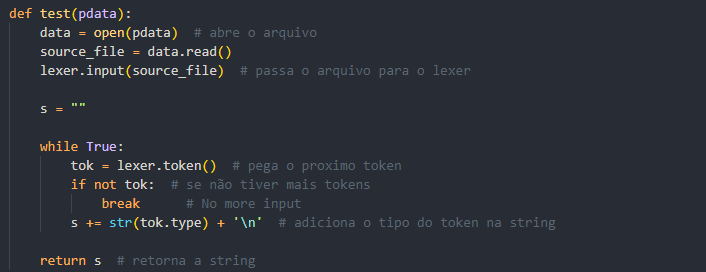
\includegraphics[scale=0.8]{images/varredura.png}
        \label{fig:f2}
        \end{figure}	

\subsection{Reconhecimento de tokens}
A identificação de tokens é feita pelo ply, que é uma biblioteca para análise léxica e sintática. Utilizamos dentro do código um vetor tokens, que contém todos os tokens que serão reconhecidos pelo analisador léxico. O bloco de código na Figura \ref{fig:f3} mostra a lista de tokens.

 
      \begin{figure}[h!]
        \centering
         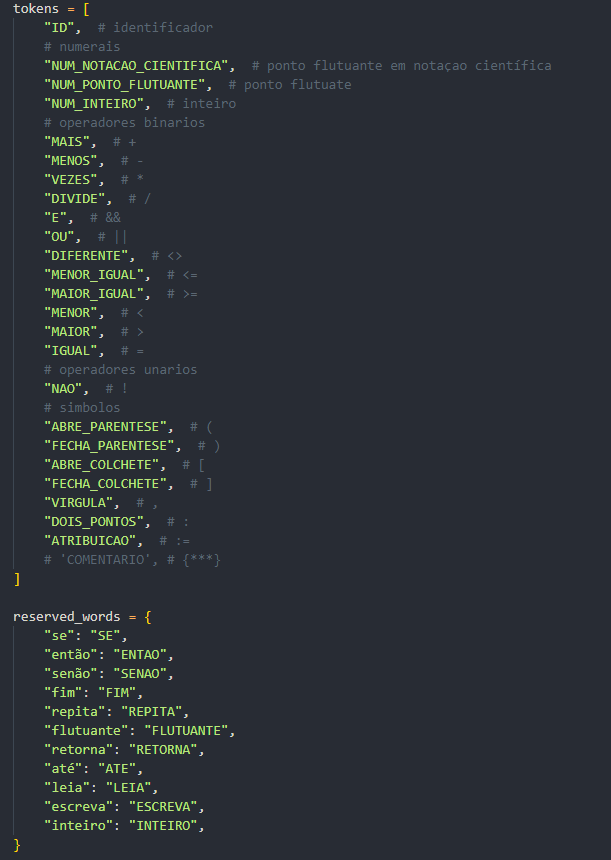
\includegraphics[scale=0.8]{images/tokens.png}
        \label{fig:f3}
        \end{figure}

\subsection{Detecção de erros}
A detecção também é feita pelo ply, porém a organização da mensagem de erro é feita pelo código. O bloco de código na Figura \ref{fig:f4} apresenta a implementação da detecção de erros. Além do erro, ele também apresenta a linha e a coluna onde o erro ocorreu.

 
      \begin{figure}[h!]
        \centering
         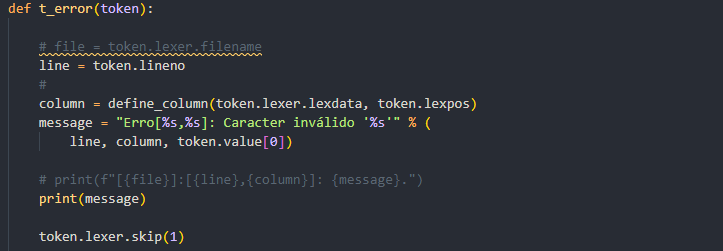
\includegraphics[scale=0.8]{images/erros.png}
        \label{fig:f4}
        \end{figure}



\section{Execução}

\subsection{Execução do analisador léxico}
Para executar o analisador léxico, basta executar o arquivo \textbf{tpplex.py} dentro da pasta de \textbf{implementacao}. O arquivo aceita dois parâmetros, o primeiro é o arquivo de entrada, e o segundo é o arquivo de saída. O arquivo de entrada deve ser um arquivo com extensão \textbf{.tpp}, e o arquivo de saída deve ser um arquivo com extensão \textbf{.out}.

Abaixo, temos um exemplo de execução do analisador léxico, onde o arquivo de entrada é \textbf{verifica_valor_10.tpp} e o arquivo de saída é \textbf{verifica_valor_10.tpp.out}.

\begin{ lstlisting}[language=Python]
  ID
  ABRE_PARENTESE
  INTEIRO
  DOIS_PONTOS
  ID
  FECHA_PARENTESE
  INTEIRO
  DOIS_PONTOS
  ID
  ABRE_COLCHETE
  NUM_INTEIRO
  FECHA_COLCHETE
  Erro[3,19]: Caracter inválido ';'
  INTEIRO
  DOIS_PONTOS
  ID
  ID
  ID
  ATRIBUICAO
  NUM_INTEIRO
  ID
  Erro[7,20]: Caracter inválido '©'
  ID
  MAIOR
  NUM_INTEIRO
  ID
  Erro[7,31]: Caracter inválido '§'
  ID
  ID
  ABRE_COLCHETE
  ID
  FECHA_COLCHETE
  ATRIBUICAO
  ID
  Erro[9,18]: Caracter inválido '%'
  NUM_INTEIRO
  ID
  ATRIBUICAO
  ID
  DIVIDE
  NUM_INTEIRO
  FIM
  INTEIRO
  DOIS_PONTOS
  ID
  ID
  ATRIBUICAO
  ID
  MENOS
  NUM_INTEIRO
  REPITA
  ESCREVA
  ABRE_PARENTESE
  ID
  ABRE_COLCHETE
  ID
  FECHA_COLCHETE
  FECHA_PARENTESE
  ID
  ATRIBUICAO
  ID
  MENOS
  NUM_INTEIRO
  ID
  Erro[22,8]: Caracter inválido '©'
  ID
  MENOR
  NUM_INTEIRO
  FIM
  INTEIRO
  ID
  ABRE_PARENTESE
  FECHA_PARENTESE
  INTEIRO
  DOIS_PONTOS
  ID
  LEIA
  ABRE_PARENTESE
  ID
  FECHA_PARENTESE
  ID
  ABRE_PARENTESE
  ID
  FECHA_PARENTESE
  ID
  ID
  IGUAL
  NUM_INTEIRO
  ID
  ABRE_PARENTESE
  NUM_INTEIRO
  FECHA_PARENTESE
  FIM
\end{ lstlisting}




\bibliographystyle{sbc}
\bibliography{sbc-template}




\end{document}